
\cleardoublepage


\chapter{Experimental Validation}


\section{Introduction}

% -------------------------------------------------------------------------------------------
\section{Modeling}

\subsection{NEBP Decoupling}

% why model?
Before conducting any flux measurement of the beam port, the experimental setups were first modeled in MCNP.
The purpose of this is twofold: one, this generates predictive detector responses to aid in the selection of experimental parameters and provides a metric for the accuracy of initially measured results, and two, response functions are generated for the devices that are ultimately used in the unfolding of the final spectrum.
% can i use the full model?
However, due to the (computational) size of the full reactor model, it would be very expensive to generate these experimental responses and response functions.
Also, the beam port flux, not in-core source spectrum is what we desire to measure, so the response functions would not relate back to the proper flux using the full model.
% no, we need a decoupled model
Necessarily, a decoupled model of the beam and experimental configurations must be used for this portion of the simulation.
This will simplify the geometry and transport significantly, allowing for reduced computation times and also for the ultimate unfolding of the correct neutron spectrum.
% is it valid to decouple?
As to the validity of this decoupling, as long as the full surface current leaving the outer boundary of the full model is captured in the decoupled model, then this approach is neutronically equivalent to a non-decoupled approach.
% yeah, as long as the coupled surfaces capture the outgoing flux, in our case that's justified because a vast majority comes down the beam
In our case, as indicated by the flux results from the previous chapter, the vast majority of departing neutrons leave the beam through the collimator void.
The tallies include a large area around this beam, too, to account for any neutrons that escape the beam.
This flux value decreases rapidly further from the center of the beam, and so it is believed that any neutrons that escape the collimator, leave through the structural material around the collimator, and still manage to interact in any detector will contribute in a statistically insignificant way.

% what does the decoupled model include?
The decoupled model includes the 8" outer portion of the NEBP, which would account for any backscattering from either detector.
% well, i converted the tally into a source at the surface 
The tally from the full model was converted into a steady-state source placed at the outer face of the NEBP.
% the beam and space outside contain universes that different detectors can be included in
The collimator void and space outside of the NEBP contain universes that allow different detectors to be swapped in and out of the model.
% the whole thing is wrapped and driven by python, too so that's great
The entire decoupled model is wrapped in python to allow for variation in input parameters and for the easy extraction and processing of output data.


\subsection{Gold Foil Tube}

% the foil tube was a type of spectrometer
The gold foil tube is a kind of neutron spectrometer.
% the gold foil tube design was based on the bonner sphere - thermal responsing detector with varying moderation
In design, it is principally based on the bonner sphere spectrometer.
Gold foils, which preferentially absorb thermal neutrons are spaced with sections of high density polyethylene (HDPE).
% produce independent responses
HDPE is a strong neutron moderator, meaning that the response of each foil will be somewhat independent of the others, since neutrons are slowing down and being absorbed between foils.
% it was also meant to help with beam alignment and to simplify the beam characterization process
This design also is advantageous in that it solves issues with beam alignment and only requires a single irradiation to generate multiple responses.

%
%\begin{figure}[htb]
%\centering
%\includegraphics[height=4in]{tex/figures/.png}
%\caption[]{}
%\label{fig:}
%\end{figure}


% you can see the device in FIG
The gold foil device can be seen in FIG.
% there are three major components, the aluminum tube, the hdpe separators and the gold foils
The tube is comprised of three separate materials, the gold foils, the HDPE separators, and the aluminum containment tube.
% the gold foils are __ diameter and __ thickness
Each of the gold foils are 5$mm$ in diameter and 0.1$mm$ thick.
% the hdpe was cylinders of __ size
The HDPE sections were 1" thick cylinders.
% each hdpe piece had a __ size hole drilled into it where the gold foil would be situated
A 1$mm$ depth, 5$mm$ OD hole was drilled into the front of each section where the gold foil was situated.
% all of these would be encased in __ID __OD aluminum tubing
All of these sections were sandwiched together and encased in 0.75" OD, 1/24" thick aluminum tubing.
% aluminum is chosen because it's relative insensitivity towards neutrons
Aluminum was chosen because of its relative insensitivity to neutrons.
% the whole apparatus had __ hdpe pieces and foils, with the first foil being exposed and a gap of __ at the beginning
The whole apparatus was comprised of 12 HDPE pieces and foils, with the first, exposed foil being situated 1" from the start of the tubing.

% this device was modeled in mcnp, where f4 flux tallies, folded with the au n,g response were used with a scx card to produce the rfs
This device was modeled in MCNP, where f4 flux tallies, folded with the $^{198}$Au(n,$\gamma$) cross sections were used with an SCX card to produce the response functions.

\subsection{Bonner Sphere Spectrometer}

% a second, active detector was included in the experiment, too, the bss
A second, active detector was also used in the spectrometric section of the NEBP analysis, too, the Bonner Sphere Spectrometer (BSS).
% the bonner sphere spectrometer uses a series of plastic spheres surrounding a lithium iodide detector to produce independent responses
The bonner sphere, while explained more thoroughly in chapter 2, use a series of plastic sphere surrounding a LiI detector to produce independent neutronic responses.

%
%\begin{figure}[htb]
%\centering
%\includegraphics[height=4in]{tex/figures/.png}
%\caption[]{}
%\label{fig:}
%\end{figure}



% you can see the device in FIG
This device can be seen modeled in FIG.
% the full device was modeled using the 4x4 mm detection crystal coupled with pmt and hdpe sphere
The main feature of the device was the 4x4$mm$ detection crystal located at the center of the sphere, although smaller details were also captured with the model, including the photomultiplier tube and some of the detector casing material.
% positioned a distance of __ from the bp aperture
The device was positioned a distance of (???) from the NEBP aperture.
% rfs were generated for sphere sizes of __ __ __ whatver
Response functions were generated for the bare response, as well as the 2", 3", 5", 8", 10", and 12" spheres.
% the tally used f4 folded with the n,t reaction in the crystal with the scx card again
The F4 flux tally over the detection crystal was folded with the (n,t) reaction cross section and an SCX card was again used to produce response functions.



\subsection{Response Functions}

% describe any post processing used for these results to get the values in cm2

Post processing for the gold foil tube and BSS response functions is relatively straightforward.
The response function value for energy $j$, $R_j$, is multiplied by the number of energy groups, $n_{groups}$ and then converted from $b$ to $cm^2$.
This is because the SCX card, which allows a user to tally based on what source distribution bin a particle was born in, will naturally be weighted by the probability of a particle being born in that bin.
To generate the response functions, all bins were considered equiprobable, which means that the true result requires the simple multiplying by the number of bins.
The $cm^2$ conversion is because flux is generally understood in $cm^{-2}s^{-1}$, so using response functions in these units allows one to avoid that conversion later.

\begin{equation}
\label{eqn:postprocessing_au}
R_j = R_{j, mcnp} \times n_{groups} \times 10^{-24}
\end{equation}


% the gold foil tube response functions
\begin{figure}[htb]
\centering
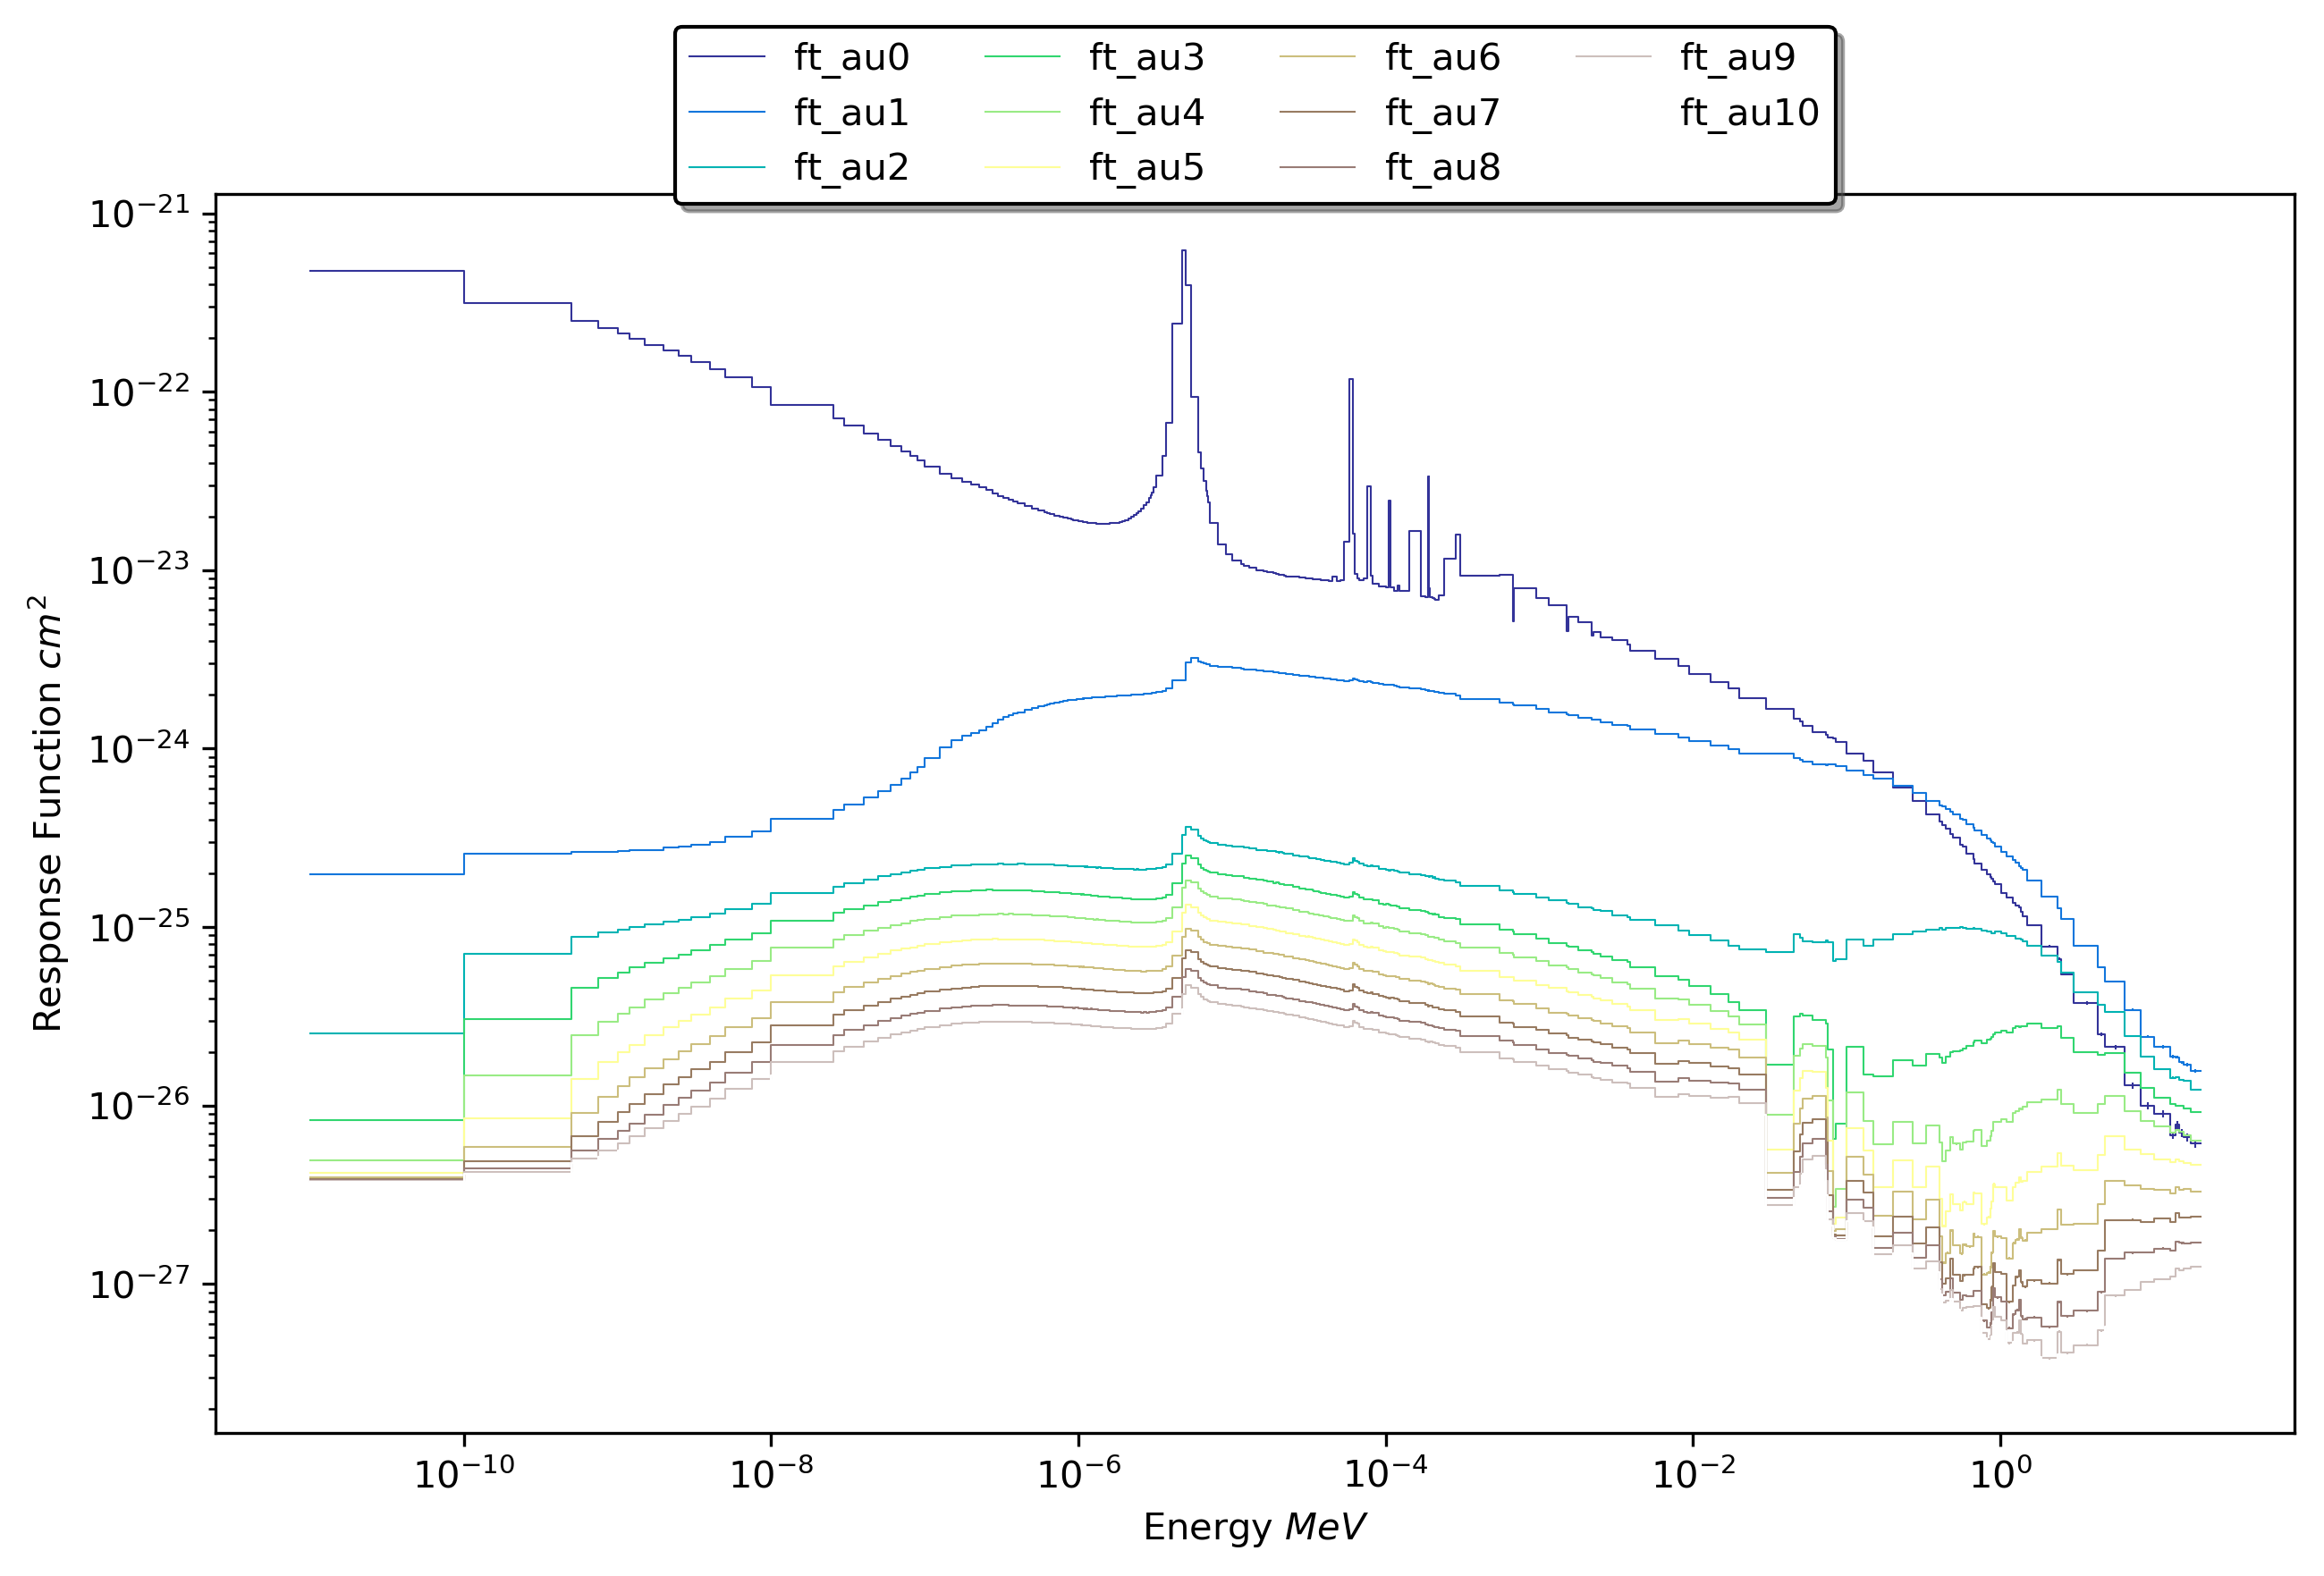
\includegraphics[height=4in]{tex/figures/ft_au.png}
\caption[Gold Foil Tube Response Functions]{The response functions for the gold foil tube.}
\label{fig:ft_au_rfs}
\end{figure}

% discuss the ft_au response functions
The response functions for the gold foil tube are pictured in \FIG{fig:ft_au_rfs}.
As distance from the tube front increases, many interesting features form and decay.
The first response very closely resembles the $^{198}$Au(n,$\gamma$) reaction, since it is exposed to the source and backscattering contributes relatively little to this response.
However, the addition of HDPE tapers the thermal tail of this response very quickly and shifts peak behavior towards the right.
The four sections that follow the first actually have an even higher response than the exposed foil.
Throughout the epithermal region, the relatively slow curvature doesn't seem much affected by the increasing foil distance, but in the fast region, a peak forms after 2", and then grows (relatively) and is pushed to the right as foil distance increases.
Overall, the goal of producing response functions that are independent was met to at least some degree with this device design.

% the bonner sphere response functions
\begin{figure}[htb]
\centering
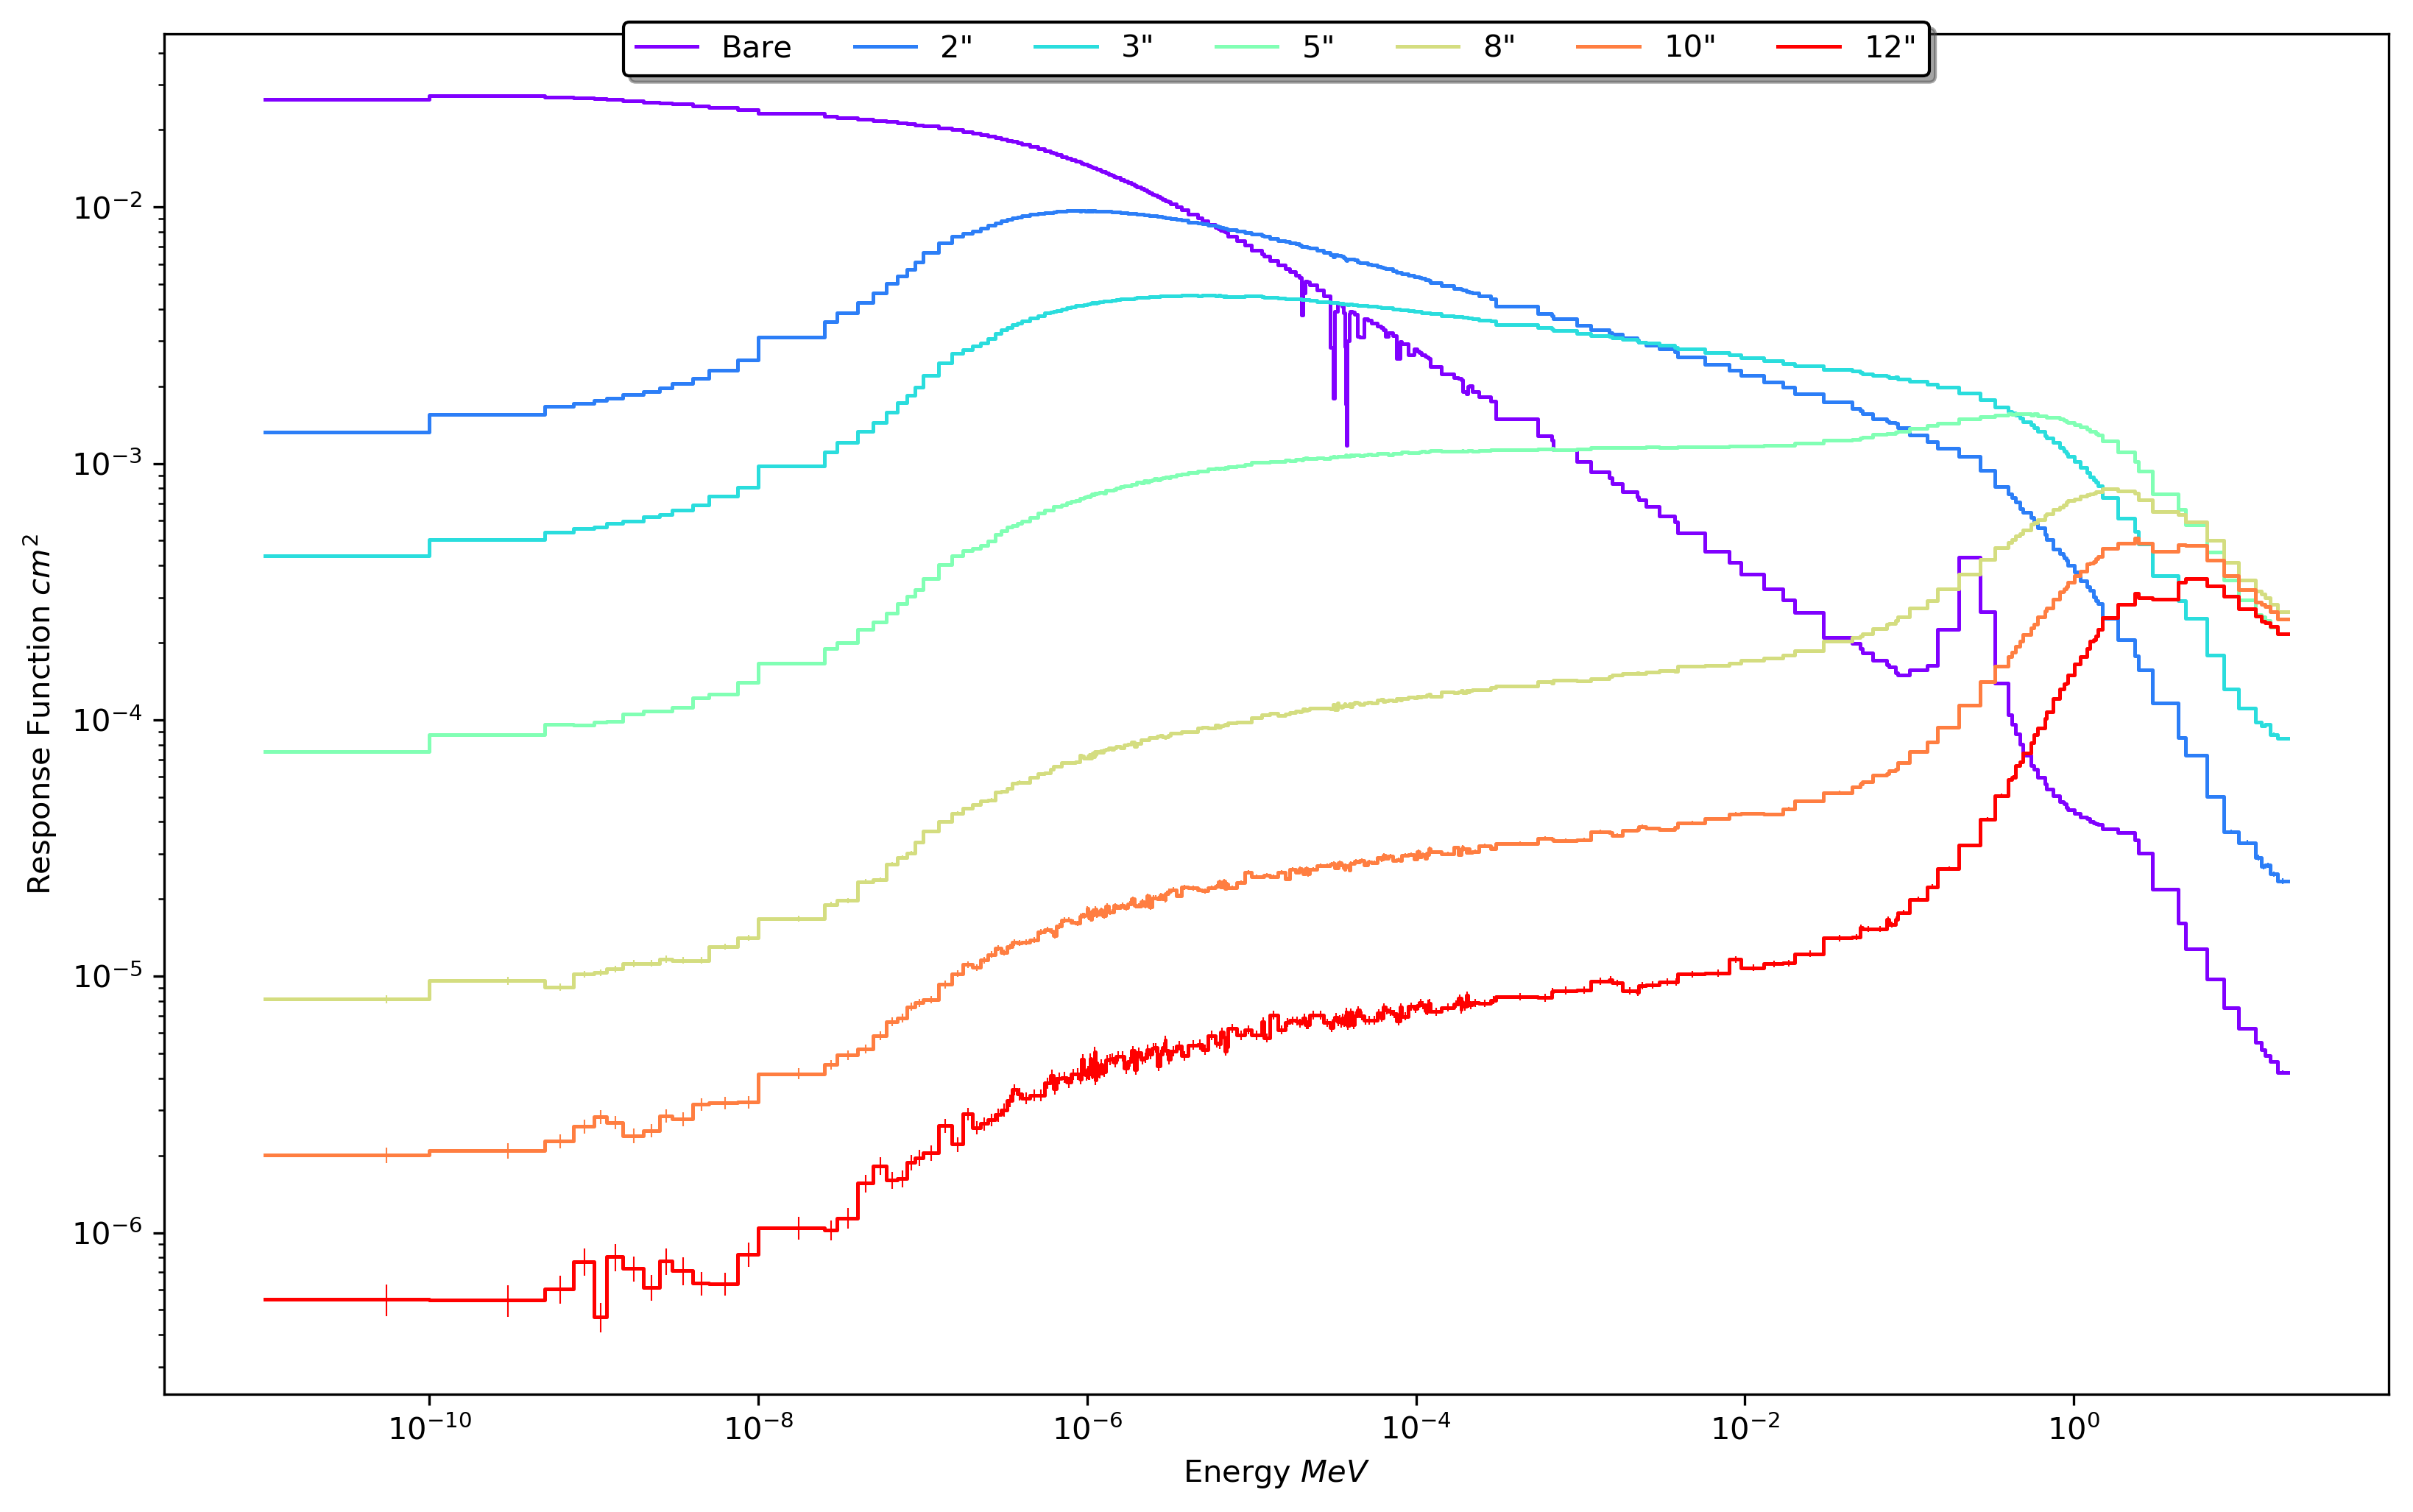
\includegraphics[height=4in]{tex/figures/bs.png}
\caption[Bonner Sphere Spectrometer Response Functions]{The response functions for the Bonner Sphere Spectrometer.}
\label{fig:bs_rfs}
\end{figure}

The trends in the BSS are similar to that of the gold foil tubes.
The bare response is thermally dominated, but as HDPE spheres are added, a peak begins to form and then is pushed towards the right.
The main difference between the two devices, besides number of detectors, is their respective responses to thermal neutrons.
Even though the thermal response is depressed in the gold foil tube, the BSS is almost completely insensitive to thermal neutrons, and there is a much larger difference between the fast and thermal response.
This is likely due to the spherical geometry used.
The BSS have lots of room around the detector for neutrons to thermalize, meaning that the fast peaks will grow to be very sharp.
In the foil tube's case, a scattered neutron is much more likely to escape the device and not be absorbed by the foil, meaning that the contribution to the fast portion of the spectrum will be much lower, relatively.

% -------------------------------------------------------------------------------------------
\section{Experimental Procedures}


\subsection{Gold Foil Tube}

% foils were individually weighed and included in table
First, the foils were individually weighted and those values are shown in \TAB{tab:au_masses}.
% the device was assembled
The device was then assembled as described in the modeling section.
% outer shielding was removed from the beam port configuration
Some of the outer shielding around the beam port was removed to access the collimator.
% the devices was attempted to fit into the beam port but deformation prevented insertion
Initially, an attempt was made to insert the device into the collimator, but deformation in the aluminum portion of the collimator prevented insertion.
% the device was ground down to fit in and inserted to where the first piece was in line with the aperture of the collimator
The first few inches of the device were then ground down with a belt sander to reduce the diameter of the device slightly.
The device was then inserted into the reactor.
% then, the reactor was powered on to __ kwth
Reactor power was brought to 100kW(th).
% the reactor remained at power for __ hours
The reactor remained at power for approximately 2.5 hours.
% then the reactor was shut down
Following the irradiation, the reactor was shut down.
% after allowing the device to cool for a bit, the individual foils were removed and bagged
A cooling period was necessary for the short-lived isotopes produced in the collimator and device to decay.
Then, the device was removed, and from the device, the individual foils were removed and bagged.
% foils were moved to an individual counting station where they were counted (gamma spec)
The foils were moved to an individual counting station, where they were sequentially counted using an HPGE.

% foil tube experimental configuration
\begin{figure}[htb]
\centering
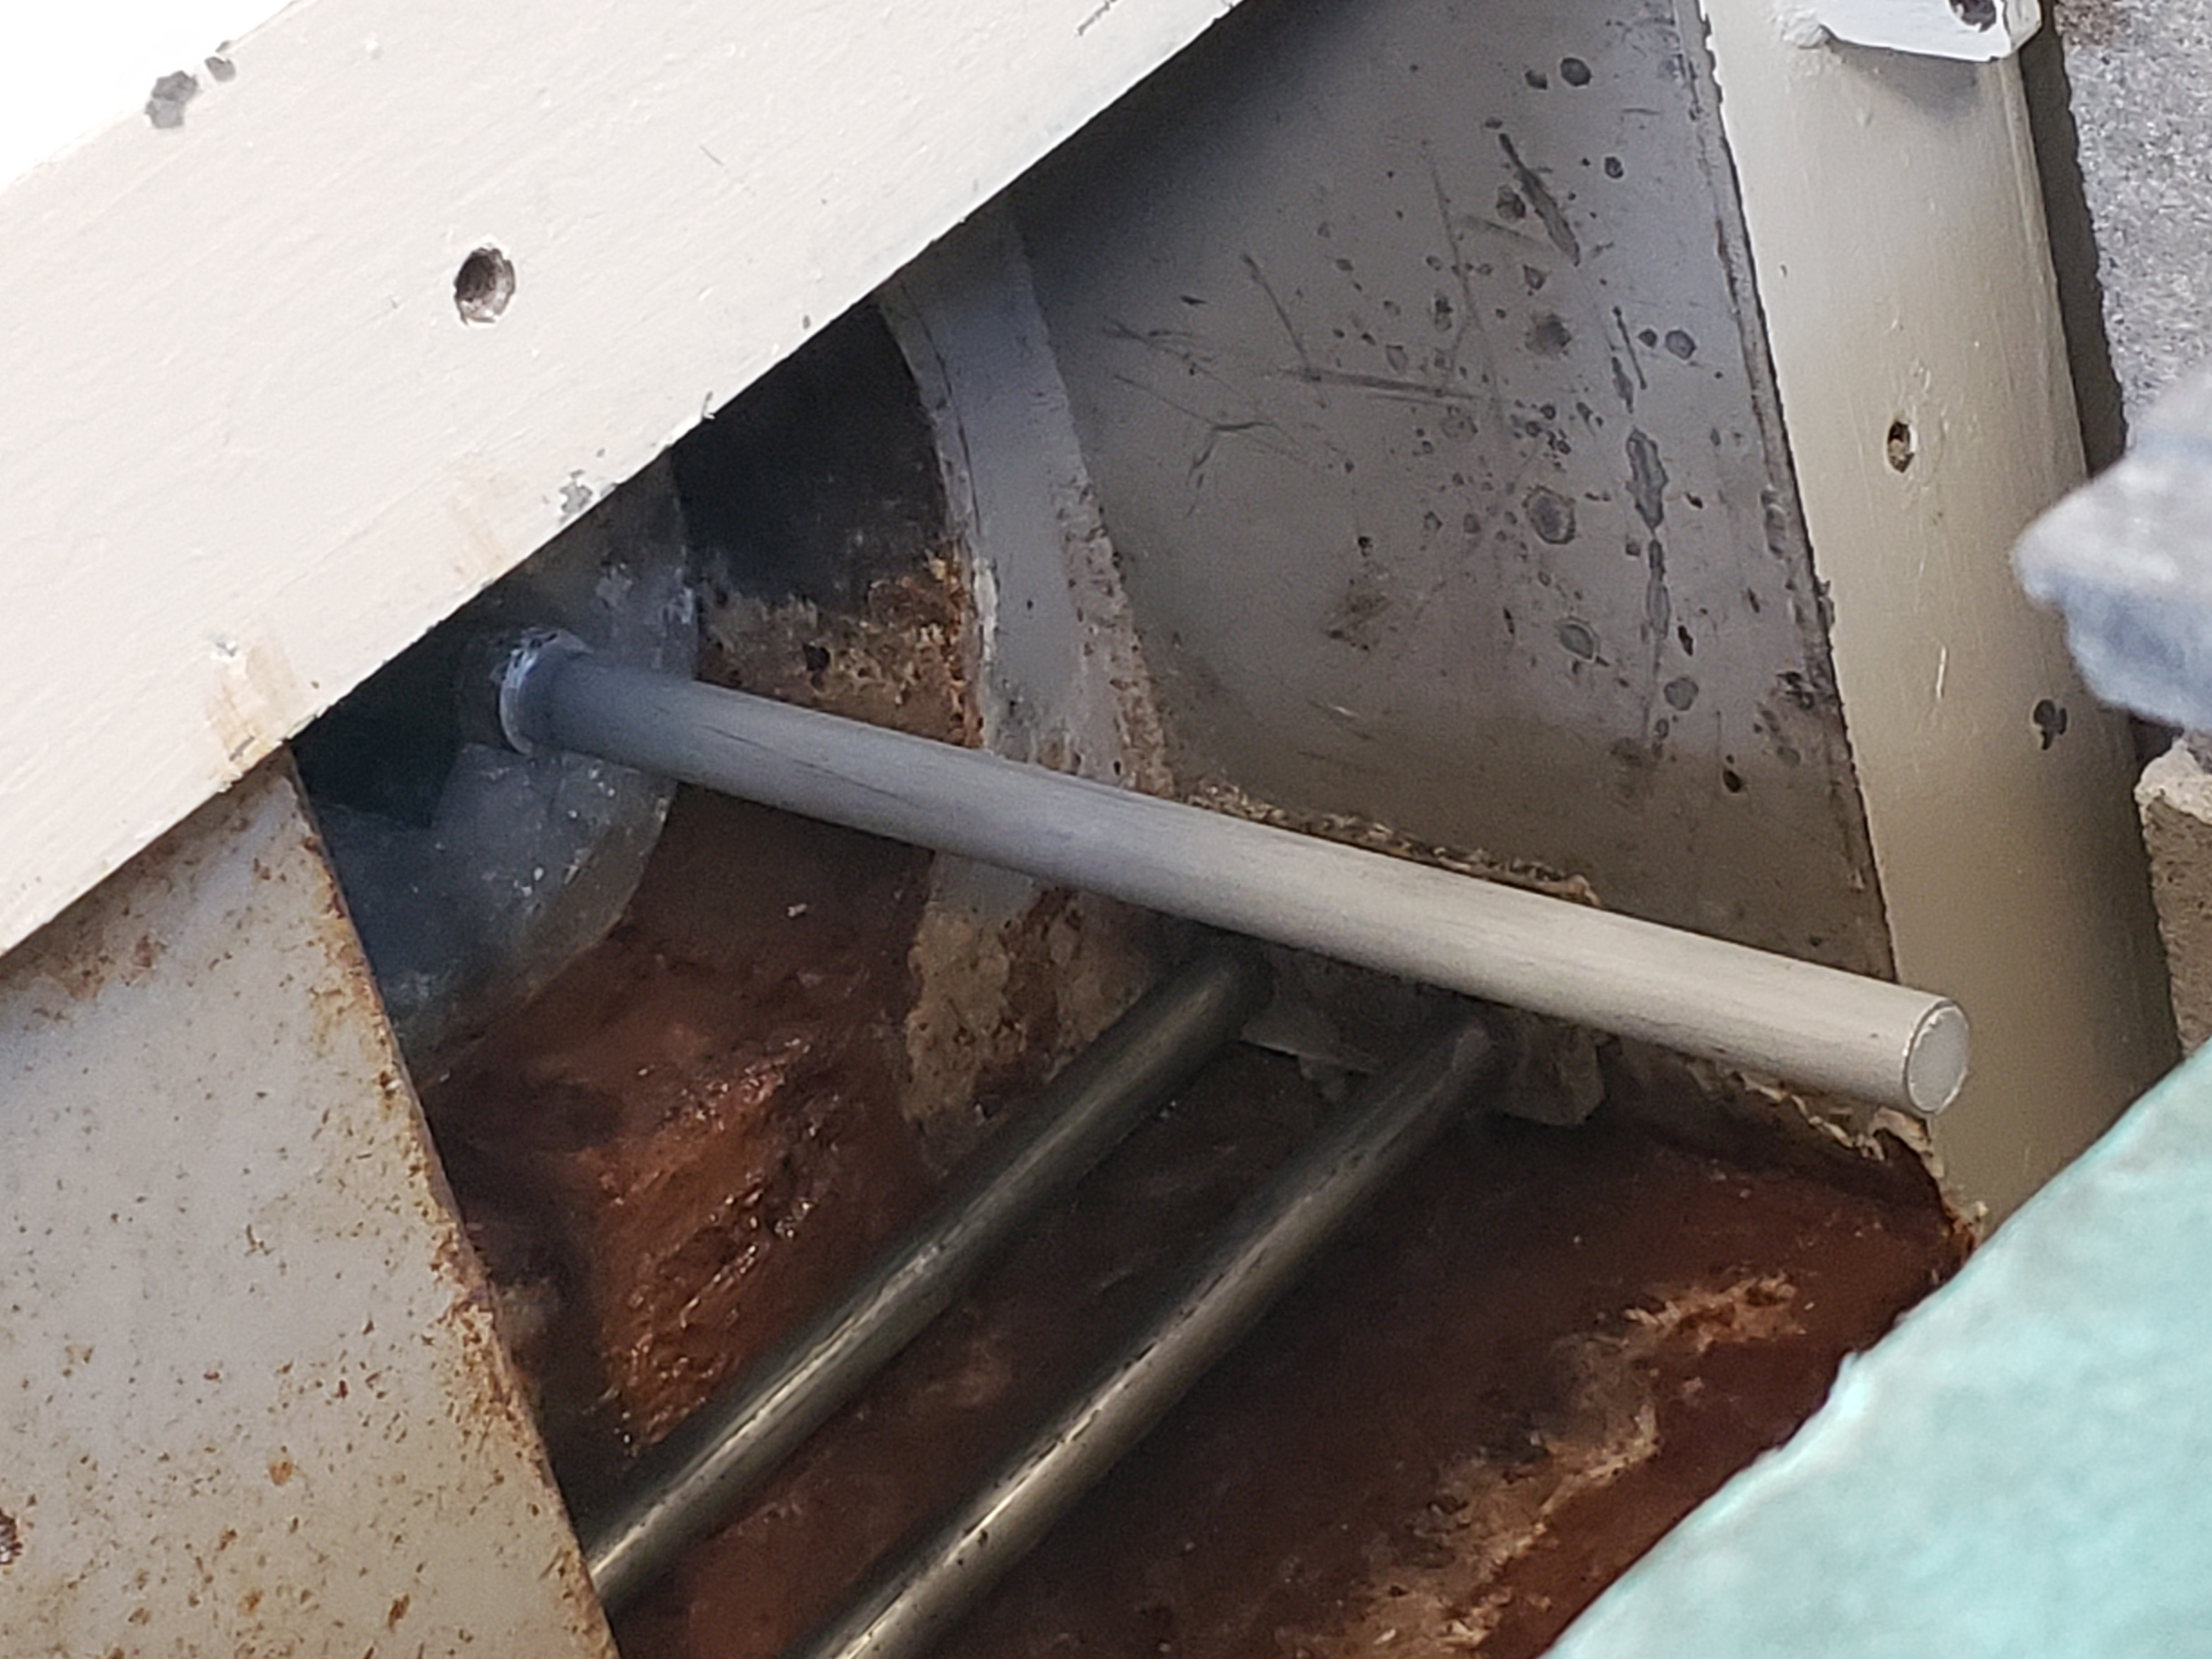
\includegraphics[height=3in]{tex/figures/ft_au_in_beam.jpg}
\caption[Gold Foil Tube Experiment]{A view of the gold foil tube inserted into the NEBP collimator.}
\label{fig:ft_au_in_beam}
\end{figure}

% this contains all of the advantg parameters
\begin{table}[h]\centering
\label{tab:au_masses}
\caption{The masses of the gold foils.}
\begin{tabular}{ r | r | l }
\toprule
Foil ID  & Position (in.)     &   Foil Mass (g)\\
2 & 0 & 0.0320\\
13 & 1 & 0.0312\\
4 & 2 & 0.0320\\
5 & 3 & 0.0318\\
6 & 4 & 0.0319\\
7 & 5 & 0.0325\\
8 & 6 & 0.0326\\
9 & 7 & 0.0320\\
10 & 8 & 0.0318\\
11 & 9 & 0.0326\\
12 & 10 & 0.0317\\
\end{tabular}
\end{table}

\subsection{Bonner Sphere Spectrometer}

% for the bonner spheres, the device was placed vertically in a manner that aligned the detection crystal with the beam at a distance of ___ cm
For the BSS irradiation, the device was positioned vertically in a manner that aligned the detection crystal with the center of the beam at a distance of (???) cm.
% the detector was set to aquire for __ s, and then the reactor was brought to __ kwth.
The detector was set to aquire for 300 s live time and then the reactor was brought to 100kW(th).
% the lld setting was adjusted to where the noise could be removed, but the lithium,T peak wasn't affected
The lld setting was electronically adjusted to reduce the detector dead time, without removing the $^6$Li(n,t) peak.
% spectra were aquired for each configuration
Spectra were aquired for the bare, 2", 3", 5", 8", 10", and 12" configurations.
For the 12" sphere, a live time of 600 seconds was used to help achieve lower counting statistics.
% the reactor was then powered off
Following the experiment, the reactor was powered off.

% ------------
% i need to put all the detection settings and stuff here
% ------------


% ------------
% also, add pictures of both setups
% ------------


% -------------------------------------------------------------------------------------------
\section{Postprocessing and Results}
\subsection{Gold Foil Tube}
\subsection{Bonner Sphere Spectrometer}

% -------------------------------------------------------------------------------------------
\section{Spectral Unfolding}
\subsection{Methods and Parameters}
\subsection{Results and Discussion}


